\section{Demonstration Setup}
At the heart of our demonstration is a web-based Top-$k$ list
extraction user interface. A screenshot of this interface is
shown in Figure \ref{fig:gui}. On this site, user can pick any
of the pre-installed benchmark data set, and execute
our extraction algorithm on the set. User can examine the original
page and the extracted output side-by-side. They can also tune the behavior
of the system by enabling or disabling various optimization and
check the outcome. The demo page also provides option to run
other algorithms such as Web tables, MDR or Ventex on the same data
set. In addition to pre-installed data, user can optionally
type in any URL and a number $k$. The system will retrieve the 
page in real time and attempt to extract the top-$k$ list from it,
or declare failure if it doesn't exist.


\begin{figure}[th]
	\centering
	\epsfig{file=./pic/Snapshot_PartA.eps,width=0.9\columnwidth}
\caption{The Top-k Extraction Web GUI}
\label{fig:gui}
\end{figure}

